% This file was converted to LaTeX by Writer2LaTeX ver. 1.4
% see http://writer2latex.sourceforge.net for more info
\documentclass[11pt]{article}
\usepackage[utf8]{inputenc}
\usepackage[T1]{fontenc}
\usepackage[french]{babel}
\usepackage{amsmath}
\usepackage{amssymb,amsfonts,textcomp}
\usepackage{array}
\usepackage{hhline}
\usepackage{hyperref}
\hypersetup{colorlinks=true, linkcolor=blue, citecolor=blue, filecolor=blue, urlcolor=blue}
\usepackage{graphicx}
% footnotes configuration
\makeatletter
\renewcommand\thefootnote{\arabic{footnote}}
\makeatother
% Text styles
\newcommand\textstyleListLabellxx[1]{#1}
\raggedbottom
% Paragraph styles
\renewcommand\familydefault{\rmdefault}
\newenvironment{styleStandard}{\renewcommand\baselinestretch{1.0}\setlength\leftskip{0cm}\setlength\rightskip{0cm plus 1fil}\setlength\parindent{0cm}\setlength\parfillskip{0pt plus 1fil}\setlength\parskip{0in plus 1pt}\writerlistparindent\writerlistleftskip\leavevmode\normalfont\normalsize\writerlistlabel\ignorespaces}{\unskip\vspace{0.111in plus 0.0111in}\par}
% List styles
\newcommand\writerlistleftskip{}
\newcommand\writerlistparindent{}
\newcommand\writerlistlabel{}
\newcommand\writerlistremovelabel{\aftergroup\let\aftergroup\writerlistparindent\aftergroup\relax\aftergroup\let\aftergroup\writerlistlabel\aftergroup\relax}
\title{}
\author{Enseignant}
\date{2020-04-02}
\begin{document}
\clearpage\setcounter{page}{1}\begin{styleStandard}
\textbf{Transcribing interlanguage: The case of verb-final [e] in L2 French}
\end{styleStandard}

\begin{styleStandard}
\textbf{Pascale Leclercq}
\end{styleStandard}

\begin{styleStandard}
\textbf{Université Paul Valéry Montpellier 3}
\end{styleStandard}

\begin{styleStandard}
\textbf{Abstract}
\end{styleStandard}

\begin{styleStandard}
This chapter aims at shedding some light on the place of transcription in the data interpretation process. More specifically, it focuses on the example of verb-final [e] in oral second-language French, which causes interpretation problems when context does not provide disambiguation cues. Through an analysis of three studies on this phenomenon (Herschensohn 2001, Prévost 2007a, 2007b, Granget 2015), displaying a variety of theoretical frameworks (generative versus functional) and transcription options (written- and spoken-centric approaches), I show that transcription choices, whether made intuitively or in a theory-constrained manner, are often problematic as they entail an early categorization of data, even before data coding and analysis, thereby introducing an interpretive bias (Mondada 2007). Finally, I draw some conclusions and offer suggestions regarding best transcription practices. 
\end{styleStandard}

\begin{styleStandard}
\textbf{Keywords:} transcription, data interpretation, L2 French, verbal morphology, interlanguage
\end{styleStandard}

\begin{styleStandard}
\textbf{1. Introduction}
\end{styleStandard}

\begin{styleStandard}
This chapter stems from the author’s questions and doubts while engaging in corpus-based second language acquisition (SLA) research, and more specifically when facing oral learner production that is ambiguous and requires the researcher to make conscious transcription decisions. I was particularly puzzled by the way some English learners of French use verb-final [e] as a generic verb ending, in spite of its highly polysemous value (e.g., \textit{tomber} ‘fall’ infinitive, \textit{tombait} ‘was falling’ imperfect, \textit{tombé} ‘fallen’ past participle, etc.) and wondered how to transcribe and to interpret such forms. This phenomenon has been pointed out regularly over the last decades in the literature on the acquisition of morphosyntax and has been studied from a variety of theoretical perspectives (Myles et al. 1998, Herschensohn 2001, Bartning \& Schlyter 2004), making it an interesting case for a study on the links between interlanguage description and interpretation (see for example the negation phenomenon, Ortega 2014). The description of learner language is indeed a complicated business, which involves, to a certain degree, inferring what learners want to say in a given context. How do researchers deal with this when transcribing raw data? How do they make such inferences? To what extent are their choices theory constrained? This paper aims at shedding some light on these issues.
\end{styleStandard}

\begin{styleStandard}
The concept of interlanguage (Selinker 1972, Han \& Tarone 2014, Pallotti 2017) is key in SLA, as it reflects that a learner’s language is a system in itself, and one which can vary in time and in contexts of use according to a number of variables (e.g., length and type of instruction, time spent in the target language country, motivation, aptitude, socioeconomic background, linguistic context, interlocutor). It depicts the language of learners as a dynamic unstable system, influenced by the patterns of the source language and/or other known languages, stabilizing at times, and sometimes subject to attrition or fossilization. Interlanguage development (notably speed and level of achievement) is constrained at the level of the individual, yet many researchers believe that there are shared itineraries (e.g., Bartning \& Schlyter 2004), although this by no means implies that all developmental paths are the same. Researchers endeavouring to identify the dynamics of learning a language are faced with crucial methodological choices, regarding study design, data transcription and theoretical framework (Mackey \& Gass 2012, Révész 2012). In particular, they have to pay close attention to individual performance so as to find patterns, which may point to some general, and possibly universal, learning processes. Consequently, following Selinker’s (1972) admonition to describe interlanguage before engaging in an explanatory process, SLA researchers have been working to map as accurately as possible the way learners of a new language develop their oral and written skills, whether in production or in comprehension (Ortega 2014). Oral production offers privileged access to the processes learners are engaged in when they utter messages in a foreign language, whatever their proficiency level: The repetitions, hesitations, reformulations that are typical of the oral modality may tell the researcher whether the learners are able to plan and structure their discourse and utterances, through more or less automatized access to the second-language (L2) lexicon and grammar, and whether they are able to monitor their speech for errors (Segalowitz, 2010:47 cited by Hilton 2014:29, Kormos 2006). 
\end{styleStandard}

\begin{styleStandard}
This brings us to a major issue facing the SLA researcher: The interpretation of oral interlanguage data, a process in which transcription plays a major part. As acknowledged by Ochs (1979) in her pioneering article, and much later by Mondada (2000, 2002, 2007), transcription is a theory-laden interpretive procedure, which incorporates the researcher’s theoretical assumptions in the way oral phenomena should be represented and converted to written form. 
\end{styleStandard}

\begin{styleStandard}
Although transcription procedures are at the very heart of research on spoken language, the transcription process itself has seldom been explored, and even less so from an SLA perspective. Yet, when transcribing learner oral production, the researcher has to make a series of strategic decisions regarding how to interpret ambiguous forms, such as, for example, verb-final [e] in L2 French, which can stand for homophonous infinitive (\textit{tomb}\textbf{\textit{er}}), imperfect (\textit{tomb}\textbf{\textit{ais, }}\textit{tomb}\textbf{\textit{ait}}), past participle (\textit{tomb}\textbf{\textit{é}}\textit{,}\textbf{\textit{ }}\textit{tomb}\textbf{\textit{és}}), or passé simple (\textit{tomb}\textbf{\textit{ai}}) marks in standard French, or it might even stand for something else in the learner’s interlanguage, such as simple present (Granget 2015). How should such forms be represented in transcription? Should \ researchers use orthographic conventions and take a decision based on context and their knowledge of the target-language norms (for example, a past adverbial may lead researchers to adopt the interpretation of imperfect or \textit{passé composé}), or should they leave the interpretation open and use phonetic transcription (MacWhinney 2000:19, Saturno 2015)? 
\end{styleStandard}

\begin{styleStandard}
Against this backdrop, I purport to explore the way verb-final [e] in L2 French has been transcribed and analysed in two theoretical perspectives, with the aim of contributing to the current discussion on interlanguage description and interpretation (Ortega 2014), as well as offering some methodological reflections on data transcription. 
\end{styleStandard}

\begin{styleStandard}
Keeping in mind MacWhinney’s (2000:19) warning that “perhaps the greatest danger facing the transcriber is the tendency to treat spoken language as if it were written language”, I introduce the V-[e] transcription problem, and I reflect on the task the transcriber faces as well as on the use of the French writing system to transcribe oral learner data. Then I present the transcription, coding and interpretation choices made by three researchers (Herschensohn 2001, Prévost 2007a,b, Granget 2015) regarding the use of verb final homophonous [e] in L2 French. These three studies were selected as they feature an in-depth analysis of the [e] phenomenon, while offering different theoretical perspectives and transcription strategies (orthographic or phonetic). Based on these three approaches, and following Ortega (2014), I conclude by discussing the link between the choice of theoretical perspective and the description of linguistic data through the transcription process and providing a few guidelines for transcribers.
\end{styleStandard}

\begin{styleStandard}
\textbf{2. The verb final [e] problem in transcription}
\end{styleStandard}

\begin{styleStandard}
My first encounter with verb final [e] took place when I was preparing a paper on how learners’ way of referring to time and space in narrative discourse developed over the course of L2 acquisition and whether the data corroborated the Aspect Hypothesis (Leclercq 2011).
\end{styleStandard}

\begin{styleStandard}
Through a focus on motion predicates, in combination with tense and aspect markers, and within a crosslinguistic perspective, I wanted to provide a characterization of elementary, intermediate and advanced proficiency levels. The main research question was the following: How do learners’ ways of referring to time and space develop over proficiency levels? I hypothesized that the selection of motion predicates was closely linked to morphological aspect marking (aspect hypothesis, Andersen \& Shirai 1994, Robison 1995, also see Rohde 1996 for an overview), and that ambiguous forms as regards tense/aspect marking in English would decrease over proficiency levels.
\end{styleStandard}

\begin{styleStandard}
The experimental design consisted of the administration of a biographical questionnaire, which included information regarding the language-learning history of the participants, and the completion of the Horse Story, an oral picture-based story-telling task developed within the Langacross project (a Franco-German research project funded by the French National Research Agency (ANR) and supervised by Maya Hickmann). The stimulus featured five pictures in which three entities (a horse, a cow and a bird) were localized with reference to a meadow and a fence. It triggered the retelling of motion events (running, jumping, falling, flying) (see Appendix A). It was initially used to study the acquisition of spatial reference in first-language (L1) and L2 French, Chinese, German and English (Hendricks 1998, Hickmann, Hendricks \& Roland 1998). The retellings were recorded and later transcribed by a trained researcher using CLAN conventions and the recommendations provided by the Langacross team in their coding manual (Hickmann et al. 2011), after which I checked them myself. In accordance with those recommendations, a @G line was inserted in the transcriptions to indicate the correspondence between the learners’ utterances and the picture from the stimulus. For the purpose of the present chapter, the target verb final [e] forms are bolded in the following transcription.
\end{styleStandard}

\begin{styleStandard}
I now examine example (1), which presents a retelling by an intermediate-level English learner of French, Mag, including verb-final [e] forms. I highlighted those forms in the transcription. 
\end{styleStandard}

\begin{styleStandard}
(1) Horse Story, 2011 transcription, English L1, French L2 Mag, intermediate.
\end{styleStandard}

\begin{styleStandard}
@G:\ \ pict\_1
\end{styleStandard}

\begin{styleStandard}
*SUJ:\ \ \textit{dans une première c' est un cheval }. ‘in a first it is a horse’
\end{styleStandard}

\begin{styleStandard}
*SUJ:\ \  \textit{qui court dans une prairie }. ‘which runs in a meadow’
\end{styleStandard}

\begin{styleStandard}
@G:\ \ pict\_2
\end{styleStandard}

\begin{styleStandard}
*SUJ:\ \ \textit{mm c' est mm une vache dans le prochain image }. ‘it is a cow in the next picture’
\end{styleStandard}

\begin{styleStandard}
*SUJ:\ \ \textbf{\textit{séparée }}\textit{par une mm un pré mm avec un oiseau }. ‘separated by a field with a bird’
\end{styleStandard}

\begin{styleStandard}
@G:\ \ pict\_3
\end{styleStandard}

\begin{styleStandard}
*SUJ:\ \ \textit{mm alors dans le troisième le cheval }\textbf{\textit{essayE }}\textit{de monter le }. ‘so in the third the horse try to climb the’
\end{styleStandard}

\begin{styleStandard}
*SUJ:\ \ \textit{comment on dit} . ‘how do you say’
\end{styleStandard}

\begin{styleStandard}
\ *EXP:\ \ \textit{la barrière .} ‘the barrier’
\end{styleStandard}

\begin{styleStandard}
*SUJ:\ \ \textit{la barrière oui} . ‘the barrier yes’
\end{styleStandard}

\begin{styleStandard}
*SUJ:\ \ \textit{mm mais le barrière se casse .} ‘but the barrier breaks’
\end{styleStandard}

\begin{styleStandard}
@G:\ \ pict\_4
\end{styleStandard}

\begin{styleStandard}
*SUJ:\ \ \textit{dans le quatrième }\textbf{\textit{est}}\textit{ le cheval }\textbf{\textit{tombE}}\textbf{ }. ‘in the fourth is the horse fall’
\end{styleStandard}

\begin{styleStandard}
@G:\ \ pict\_5
\end{styleStandard}

\begin{styleStandard}
*SUJ:\ \ \textit{et dans xxx le vache et l' oiseau euh }\textbf{\textit{aidE }}\textit{le cheval avec une boite {\textless}de{\textgreater} [/] \# de aide et \# une bandage .} ‘and in xxx the cow and the bird help the horse with a box of help and a bandage’
\end{styleStandard}

\begin{styleStandard}
What the learner produces is several instances of verbal forms with a verb-final [e] sound, which could either stand for an infinitive, or a past participle, or an inflected form (imperfect \textit{aidait} ‘helped’ for example), or which could constitute a base form in the learner’s interlanguage. What is interesting is that this particular learner used the [e] ending on a regular basis, but also used targetlike verb forms like present tense \textit{se casse} ‘breaks down’. The researcher, when facing forms that are ambiguous, has to make decisions regarding transcription and interpretation of data. 
\end{styleStandard}

\begin{styleStandard}
Example (1) shows that I chose to use regular orthographic spelling when phonological forms seemed to match the tense/aspect/person agreement rules, as is the case with \textit{séparée} ‘separated’ on line 4 of the transcription, and the V-E symbol only for the forms which I identified as potentially ambiguous, either due to a position in the sentence that might be interpreted as necessitating an inflected verb (either present tense \textit{aide} with a mute final {\textless}e{\textgreater} or passé composé \textit{a aidé }‘helped’), or due to unusual word order (\textit{est le cheval \&tombE} ‘is the horse fall-ED’). In this project I did not even consider that forms like \textit{séparée} ‘separated’ could actually be non-targetlike in the mind of the learner, and based on our knowledge of French graphonemics, the transcriber and I assumed that learners had produced target forms (a fairly naïve and controversial position). These intuitive transcription choices could be qualified, in the words of Ortega (2014), as pre-theoretical. Mondada (2000:3) nevertheless points out that such intuitive choices are highly problematic when it comes to data categorisation and interpretation.
\end{styleStandard}

\begin{styleStandard}
We will now try to shed some light on this phenomenon by considering the transcription process itself.
\end{styleStandard}

\begin{styleStandard}
\textbf{3. Transcribing as a situated practice and a cognitive challenge}
\end{styleStandard}

\begin{styleStandard}
Although it is a fundamentally theoretical enterprise (Ochs 1979), and a crucial part of the research process, transcription is a grey zone in most studies. This is reflected in the scarcity of research on the rationale and consequences of transcribers’ choices (Mondada 2002:46). In a series of papers using Ochs’ study as a starting point and a framework for the analysis of the activity of transcription from an epistemological perspective, Mondada (2000, 2002, 2007) proposes an in-depth description of the transcription process. Bearing her analyses in mind, I discuss the practical and cognitive challenges awaiting the transcriber when it comes to the transcription of verb final [e] in L2 learner data.
\end{styleStandard}

\begin{styleStandard}
\textbf{3.1 What is transcription?}
\end{styleStandard}

\begin{styleStandard}
First, Mondada (2007) refers to transcribing as a “situated practice”, observing that it is “embedded within a series of research practices: data production, digitalization and compression, anonymization, storage and filing, representation and annotation, analysis, and so on […]. These practices configure and more radically ‘fabricate’ what we consider as ‘data’” (p. 810). She acknowledges the fact that transcripts on their own are not data since they cannot be autonomized from recordings (which constitute primary data). Transcripts are considered “secondary products of representation and annotation practices” (Mondada 2007:810-811). Transcripts and recordings complement each other, particularly when data transcription software such as CLAN is used, as they enable the linking of transcription with the original audio or video recording. While transcripts enable researchers to focus on detail for analysis, recordings provide the possibility to listen again. Mondada therefore acknowledges the evolutive nature of transcripts: The transcriber can endlessly check, revise, reformat, for a specific analysis or for editorial purposes (p. 810). Another inherent feature of transcribing is variability (both within and in-between transcriptions, as illustrated in the different treatments of \textit{séparée }and \textit{essayE} in (1)).
\end{styleStandard}

\begin{styleStandard}
On a more abstract level, Mondada (2000) describes the transcription process as an exploitation of writing resources in order to create a representation of oral discourse based on operations of filtering ‘noises’ (phenomena deemed non-meaningful by the transcriber), and of homogenisation through the use of systematic conventions (this latter point is particularly well exemplified in the CLAN and CHAT manuals, MacWhinney 2000). Mondada (2000) observes that the passage from oral to written form has consequences on the interpretability of the spoken language. On the one hand, the transcription appears as a structured account of oral speech, facilitating visual perception. On the other hand, having the possibility to listen again and again to the same recording provokes what Mondada refers to as a magnifier effect: The researcher can focus on a phenomenon which is ephemeral in real-time and might have passed unnoticed during normal conversation.
\end{styleStandard}

\begin{styleStandard}
In line with Ochs (1979), Jefferson (1996) and Saturno (2015), Mondada (2000) indicates that transcribing is an inherently interpretive activity. She also highlights what she calls the circularity problem: Numerous interpretations of phenomena are incorporated a priori in the transcription, in spite of their being the purported aim of the a posteriori analysis of this transcription. In other words, the transcription choices made by the researchers already contain their interpretative choices, making the whole research enterprise dubious.
\end{styleStandard}

\begin{styleStandard}
Mondada (2000:8) also describes the transcriber’s job as “isolating, cutting out, identifying, making identifiable the recorded forms in a clear written form.”\footnote{\textrm{ My translation.}} Some notation systems enable the highlighting of indeterminate forms. Among those systems, she mentions the use of International Phonetic Alphabet (IPA) as opposed to orthographic representation. She claims that using IPA suggests a form is deemed non-identifiable by the researcher, while an orthographic rendering indicates that the researcher has already categorized the form. The use of phonetic versus orthographic conventions shows that transcribed forms can be categorised as “more or less comprehensible (transparent or opaque), more or less standard (according to their distance with the standard), […] a social category, etc.” (Mondada 2000:8, my translation). While complete IPA transcriptions are often deemed unpractical (and are rarely seen in SLA projects), Mondada points out that the punctual use of IPA allows us to avoid selecting an orthographic form, and therefore a specific language (a crucial point in interlanguage studies), but also to visually detach the transcribed content and consequently highlight it. I will refer to the orthographic option as a written-centric approach, and to the punctual IPA option as a spoken-centric approach. Although the spoken-centric option appears as more careful, as it leaves data interpretation open, it is not always chosen by researchers. Why is that? An interesting hypothesis is that the written code deeply influences literate speakers’ representation and categorization of language units (Jaffré 2006, see below). 
\end{styleStandard}

\begin{styleStandard}
Keeping Mondada’s reflections in mind, I now focus on the choice of orthographic transcription and what it might imply for the transcriber, particularly how phonological and graphical representations may interact and be treated by the transcriber. I use the verb final [e] phenomenon as a basis for the analysis.
\end{styleStandard}

\begin{styleStandard}
\textbf{3.2 Cognitive aspects of the learner and transcriber’s task: Making the most of homophony in spoken French}
\end{styleStandard}

\begin{styleStandard}
While most practitioners and researchers agree that verb morphology, including verb-final [e] in French, is a major source of spelling confusion, whether for French children learning how to write (Brissaud \& Sandon 1999, David et al. 2006, Fayol \& Pacton 2006), for adults who master the orthographic system and use it daily, or for L2 learners in their oral and written productions (David et al. 2006, Brissaud et al. 2006, Prévost 2007a, Granget 2015), some researchers have started focusing on the impact of the orthographic experience on phonological awareness (Bassetti et al. 2015, Nimz \& Khattab 2019). According to Detey \& Nespoulous (2008:68), several studies suggest that “orthographic representations might play a role in speech perception […], at least through bidirectional activations between graphemes and phonemes […]. Hearing a lexical unit might activate an orthographic representation, which might in turn influence phonological judgements.” As a consequence, it is quite possible that experts’ interpretation of oral learner speech might be largely influenced, directly or indirectly, by spelling knowledge. The transcriber, whether a native speaker or an expert user of the target language, as is the case in (1), often tackles the data with a number of assumptions about what the learner knows about the language, including morphographic representations. 
\end{styleStandard}

\begin{styleStandard}
\textbf{3.3 Description of verb final [e] phenomenon in relation with the French spelling system}
\end{styleStandard}

\begin{styleStandard}
According to Jaffré (2006:25), a spelling system is not a mere tool used for the sake of written communication: Centuries of usage have fostered tight links between spelling forms and their users, whose perceptive abilities they have shaped and constructed. He therefore argues that beyond the strict communicative need to disambiguate homophones, their very orthographic differentiation has progressively conditioned the cognitive representations of literate users. In that context, the written code can be considered as an autonomous linguistic representation, capable of exerting an influence on spoken language, as shown by the orthographic distinction of homophones in French. Of course, such an influence is only possible in a society where written communication forms part of the essentials of daily life, and where literacy is a basic skill most citizens master, as is the case in 21\textsuperscript{st} century France.
\end{styleStandard}

\begin{styleStandard}
According to Jaffré (2006), spelling systems have two main objectives. First and foremost, they aim at representing a given language phonographically, but they also have a semiological agenda: They aim at providing a visual representation of language, with tools that enable the disambiguation of spoken forms, for them to be readable and interpretable. In that regards, the use of orthographic spelling for L2 transcriptions compels transcribers to make choices informed by their knowledge of the target language grammar. Additionally, although languages such as French and English use an alphabetic system, their spelling systems often depart from a one-to-one sound/letter relation. In that context, heterography appears as a tool to tease apart homophones. 
\end{styleStandard}

\begin{styleStandard}
The French morphological verbal system, and more specifically final [e], provides an interesting case as regards homophony and heterography, and one which poses a particular challenge to the learner. As noted by Brissaud et al. (2006), a form such as /t[281?]uve/ can be spelt in ten different ways (\textit{trouver, trouvé, trouvés, trouvée, trouvées, trouvai, trouvais, trouvait, trouvaient, trouvez}), making the native writer and the L2 learner’s task a daunting one. Under the umbrella of verb-final [e] forms, there are two types of combining morphemes: Mute endings (\textit{{}-e, -s, -t, -ent}), referring to person, gender and number; and tense, aspect and morphemes (among others, \textit{{}-ai, -é, -er}, respectively referring to imperfect, perfect and infinitive). Context plays a major role in the selection of the appropriate lexical item, and as a result, the appropriate spelling. However, it is often not sufficient to disambiguate homophonous conjugated verbs, as is the case between infinitive \textit{jouer} and past participle \textit{joué}, which are a frequent source of spelling mistakes, even among French native speakers. Scriptors then have to rely on their knowledge of grammatical rules to select the right target form (David 2006, Brissaud et al. 2006). Regarding verb-final [e], French scriptors have usually received explicit instruction at school as to verb-agreement rules (subject-verb agreement, and tense/aspect endings), grammatical functions and categories (such as infinitive and past participle), and linguistic manipulations to disambiguate homophonous forms (for example, if /ale/ can be replaced by /partir/, it has to be an infinitive form spelt \textit{aller}.) They may also rely on their memorization of frequent co-occurring units (for example, \textit{pour} is usually followed by an infinitive form, see Brissaud et al. 2006: 78). In a written-centric approach, the transcriber’s interpretation of ambiguous oral forms consequently requires an analysis of context, and it taps into their phraseological knowledge as well as their knowledge of the target language orthographic rules, in order to apply the relevant contextual, categorical or morphological rules.
\end{styleStandard}

\begin{styleStandard}
\textbf{3.4 A challenge for the researcher}
\end{styleStandard}

\begin{styleStandard}
When transcribing learner data, using a written-centric approach is a leap of faith, as there is no guarantee at all that the learners master the system in the same way as a native speaker. Transcribing then becomes a game of inference: The researcher tries to infer what the learner had in mind when uttering a given phrase, and makes hypotheses regarding their choices, possibly in accordance with the selected theoretical framework of analysis. Transcription problems are consequently inherent to the fact that transcribers often assume that learners share their knowledge of the target language, including its writing system. Flavell (1977, cited by Nickerson 1999:739) observes that “we are usually unable to turn our own viewpoint off completely when trying to infer the other’s, and it usually continues to ring in our ears while we try to decode the other’s. It may take considerable skill and effort to represent another’s point of view accurately through this kind of noise, and the possibility of egocentric distortion is ever present.” It is therefore important for the researcher to keep in mind that they do not know the extent of the L2 learner’s knowledge of the target language and culture. Shared knowledge, and an understanding of what the interlocutor knows, is at the heart of the communication process (Nickerson 1999, Keysar et al. 2003). We assume our interlocutors share basic communication principles. However, as Nickerson (1999) puts it, “overimputation” of one’s knowledge (i.e., attributing learners’ knowledge about the target language that they do not necessarily possess), or lack of ability to adopt another perspective than one’s own, can cause communication difficulties and lead to wrong interpretation of the interlocutor’s message. The researcher has to be careful about “overimputation” and has to remember that nothing can be taken for granted in the realm of L2 acquisition. We cannot assume that an L2 learner thinks in the exact same way as a native speaker, nor that they use verbal forms with the same degree of mastery of form/function relations. When learners use verb-final [e] forms, do they try (with mitigated success) to retrieve targetlike morphology, or do they create a new ending to compensate for their lack of procedural knowledge? When in doubt, using a spoken-centric approach (i.e., using IPA to transcribe ambiguous forms) might be a good option, as it does not entail early categorisation of the data.
\end{styleStandard}

\begin{styleStandard}
Keeping this in mind, we will examine how verb-final [e] was transcribed and analysed in three different studies (Herschensohn 2001, Prévost 2007a, 2007b,\footnote{\textrm{ Prévost (2007a) and (2007b) present complementary information about the study under consideration in this chapter.}} Granget 2015), displaying a variety of theoretical frameworks (generative vs functional) and transcription options (written and spoken-centric approaches), so as to shed light on the link between data transcription and interpretation, and offer reflections regarding best transcription practices.
\end{styleStandard}

\begin{styleStandard}
\textbf{4. Making theoretically informed transcription and interpretation choices}
\end{styleStandard}

\begin{styleStandard}
As stated by Ortega (2014: 186), “the formal linguistic study of L2 development puts theory first and is driven by the quest to understand the role that Universal Grammar or abstract linguistic knowledge plays in the acquisition of human language across the life span.” Generative researchers therefore favour a top-down approach, with overarching research questions focusing on finding proof in favour of (or against) the theoretical constructs under scrutiny through data analysis (Lardiere 2012). Data are used to inform or contradict theoretical premises. This is the case with L2 morphosyntax and particularly with the development of inflection (Herschenshohn 2001), which have been largely explored within a generative, theory-constrained framework (among others, Prévost and White 2000, Prévost 2007b, Herschensohn 2001, Hawkins 2004). On the other end of the theoretical spectrum, functionalist researchers (see Lenart \& Perdue 2004) take a rather bottom-up, data-driven approach: Based on learner discourse, they try to account for the way learners acquire and make use of formal linguistic levels of organisation (morphology, morphosyntax, lexicon) in a given context of use. In the words of Klein \& Perdue (1989) (cited by Lenart \& Perdue 2004), researchers have to solve “the learner’s problem of arranging words” to produce a contextually meaningful message. Functionalists have also provided detailed accounts of the verb-final [e] in French L2, through longitudinal studies (for example, studies based on the ESF project, such as Noyau et al. 1995, Véronique 2004), or cross-sectional studies (Bartning \& Schlyter 2004, Granget 2015). I compare theory-constrained approaches and data-driven approaches to see what each contributes to the debate on how to interpret, and thus transcribe, oral interlanguage productions, as regards the analysis of verb-final [e]. This section was also largely inspired by the work of Granget (2015), who paved the way for the following analysis by citing the work of Herschensohn (2001) and Prévost (2007a).
\end{styleStandard}

\begin{styleStandard}
\textbf{4.1 Theory-constrained and written-centric approaches: Defective or missing surface inflection hypothesis}
\end{styleStandard}

\begin{styleStandard}
The verb-final [e] phenomenon is presented by Herschensohn (2001) as part of a wider debate on the development of inflection in learner grammars and what it reveals about access of L2 users to Universal Grammar. Within a generative framework of analysis, Herschensohn seeks to determine whether the empirical data support theoretical claims regarding the reason why L2 learners’ verbal inflections are so often defective (i.e., not targetlike) especially at intermediate levels. She re-examines the relationship between the acquisition of morphology and functional categories: Some researchers claim that morphology and syntax are developed conjointly in the L2 grammar (co-dependence, Eubank 1993, 1994, Vainikka and Young-Scholten 1996, 1998a, 1998b cited by Herschensohn 2001), in the same way as in L1 grammar, while others reject such a link and propose that morphology and syntax develop independently (Schwartz and Sprouse 1996, Lardière 1998b cited by Herschensohn 2001). In this view, a lack of morphological marks is attributed to processing difficulties. L2 learners may display evidence of syntactic competence, but deficient morphological production because “under the Missing Surface Inflection Hypothesis, the L2er has a grammar with complete functional projections but incomplete morphology” (Herschensohn 2001:280). 
\end{styleStandard}

\begin{styleStandard}
Within this framework, Herschensohn (2001) argues that inflectional deficits (i.e., non-finite verbs, or other morphological errors) support neither the co-dependence nor the independence hypothesis. She claims that “the French data rather indicate that deficiencies in morphological mapping, not defective syntax (functional categories) are the cause of L2 failed inflection” (p. 273). What is very interesting in this paper, and which provides one of the main reasons to include it in the current analysis, is that the author explicitly motivates her choice of using the infinitival form in the transcription, making her approach a typically written-centric one. Tapping into the abundant literature on the acquisition of morphosyntax, she situated her transcription choice of attributing an infinitive value to verb-final [e] forms from the very onset of the paper: “the second language (L2) use of \textit{infinitives in contexts of obligatory tense} – amply documented and discussed in the literature […] – is of theoretical interest […]” (p. 273) (emphasis mine).
\end{styleStandard}

\begin{styleStandard}
Verb-final [e] is examined in this study based on data collected from two stay-abroad participants, Chloe and Emma, through a series of interviews that took place before, at midpoint and after their six-month period in France. The interviews include discussion of topics in the present tense, and questions that refer to past and future actions. 
\end{styleStandard}

\begin{styleStandard}
The data were transcribed by the author herself and checked by a French phonologist. It yielded “several hundred tokens of verb morphology” (Herschensohn 2001:285), among which “a number of verb errors are transcribed as infinitives, although the infinitival form is homophonous with the past participle and the \textit{vous} form of the present in most cases” (p. 286). Herschensohn explains the rationale behind her choice of transcription for these forms: “In the cases where the form is transcribed as an –er infinitive, the context clearly excludes the possibility that the inflection is a past participle” (p. 286). She provides the two examples in (2) and (3).
\end{styleStandard}

\begin{styleStandard}
(2) “\textit{A quelle heure est-ce que le musée }\textbf{\textit{ouvrer}}?
\end{styleStandard}

\begin{styleStandard}
\ \ \ \ \ \ \ At what time \ \ \ Q \ \ \ \ \ \ \ \ \ \ \ \ \ the museum to open” (p. 286)
\end{styleStandard}

\begin{styleStandard}
(3) “\textit{A quelle heure est-ce que le musée }\textbf{\textit{fermer}}\textit{~}?
\end{styleStandard}

\begin{styleStandard}
\ \ \ \ \ \ At what time \ \ \ Q \ \ \ \ \ \ \ \ \ \ \ \ \ the museum to close”(p. 286) 
\end{styleStandard}

\begin{styleStandard}
She explains this choice as coming from her interpretation of such interlanguage forms as “the regularization of the irregular infinitives \textit{ouvrir} (‘to open’)” rather than as the imperfect \textit{ouvrait} (‘it was opening’)” (p. 286). She notes that when she transcribed the [e] form as an infinitive, the other options (\textit{vous} form \textit{ouvrez}, past participle, imperfect form \textit{ouvrait}) were excluded by contextual information. The author also explicitly rejects an interpretation of those forms as occurrences of the imperfect (\textit{ouvrait, fermait}), as she claims that “the use of any tense other than present would be inappropriate” (p. 286). However, what does “inappropriate” mean in the context of a learner production? In spite of the author’s claim, it seems difficult to rule out the imperfect interpretation, which would be grammatically correct, though less expected than simple present in the cited context. This might well be a case of “overimputation” on the part of the researcher (Nickerson 1999), who might have been influenced by her knowledge of French written rules, as proposed by Jaffré (2006).
\end{styleStandard}

\begin{styleStandard}
In sum, Herschensohn (2001) showcases how theory constrains transcription and interpretation choices: The author’s decision to make theoretically informed choices regarding the spelling, and therefore the grammatical status, of final verb [e] forms, entails that these morphological forms are ascribed a specific (potentially erroneous) value even before the data description stage, thereby constraining interpretation. This is what Mondada (2000:2) refers to as the circularity problem: The researcher makes theory-informed data interpretation decisions at the transcription level and then analyses the transcribed phenomenon in the light of the same theoretical framework.
\end{styleStandard}

\begin{styleStandard}
Another example of theoretically informed labelling is provided in Prévost (2007a), in which he refers to verb-final [e] forms as “default forms” in his study on the influence of the source language verbal paradigm on morphological variability in L2 French. He describes L2 French infinitives as recurring erroneous forms used in contexts where other forms are expected in the target language (“1.a. \textit{Ah je voyager {\textgreater}à{\textgreater} [/] à des Etats {\textless}U{\textgreater} [//] Unis}.”). He notices that these forms are used in a similar way by child and adult learners, of various mother tongues (English, Turkish or Chinese), and at different proficiency levels (beginners to advanced). He also points out the fact that these forms are not the only ones that are used by learners and that they can co-exist with targetlike forms, often within the same sentence. He calls this phenomenon morphological variability. Like Herschensohn (2001), he situates his research within a generative framework, and asks whether morphological variability reflects some sort of deficiency of interlanguage grammars, especially as regards functional categories such as Infl(ection). 
\end{styleStandard}

\begin{styleStandard}
Prévost (2007b) analyses verbal errors produced by 21 Anglophone learners of French, at four proficiency levels (beginner to upper intermediate 3). He observed that learners produced infinitives in contexts where an inflected verb was expected, such as after a lexical subject, but they also used inflected forms in contexts where an uninflected form was expected, for example after a preposition, an auxiliary or another verb. Prévost (2007b:360) explains his transcription choices in the following way: “[A]n infinitival verb was considered nonfinite unless evidence of the contrary existed. In other words, verbs ending in [e], which is ambiguous between the infinitival marker –\textit{er}, the past participle marker –\textit{é}, and the second-person plural ending –\textit{ez}, were categorized as nonfinite unless they appeared with the second-person plural pronoun vous ‘you’.” Just like Herschensohn (2001), Prévost adopts a written-centric approach and does not envisage the possibility of an imperfect meaning or of another undetermined value. What is more, his explanation perfectly illustrates the fact that transcription choices imply a categorisation of data (and hence, constrain data analysis) (Mondada 2007).
\end{styleStandard}

\begin{styleStandard}
The examples provided in the paper show that at the level of transcription, the author chose the –\textit{er} infinitive ending whenever an ambiguous form occurred:
\end{styleStandard}

\begin{styleStandard}
(4) a. “\textit{Je parler avec administration} 
\end{styleStandard}

\begin{styleStandard}
\ \ \ \ \ \ \ \ \ \ \ \ \ \ \ \ \ \ \ \ \ I speak.INF with administration (Ann, G1)
\end{styleStandard}

\begin{styleStandard}
b. \textit{Ils visiter moi.} 
\end{styleStandard}

\begin{styleStandard}
\ \ \ \ they visit.INF me (Mike, G2)
\end{styleStandard}

\begin{styleStandard}
c. \textit{On aller au centre d’achats} 
\end{styleStandard}

\begin{styleStandard}
\ \ \ \ we go.INF to+mall (Jill, G3)
\end{styleStandard}

\begin{styleStandard}
d. \textit{Il retourner à la maison} 
\end{styleStandard}

\begin{styleStandard}
\ \ \ \ he return.INF to the house (Sandra, G4)”(p. 363)
\end{styleStandard}

\begin{styleStandard}
He justifies his choice by stating that similar constructions also occur with verbs of the second (\textit{ouvrir}) or third (\textit{boire}) group, as in (5) a, b, c and are also found in his data with negation as in (6): 
\end{styleStandard}

\begin{styleStandard}
\ (5) a. “\textit{Il boire} 
\end{styleStandard}

\begin{styleStandard}
\ \ \ \ \ \ \ \ \ \ he drink.INF (Edward, G1)” (p. 361)
\end{styleStandard}

\begin{styleStandard}
b. “\textit{Il prendre des vêtements} 
\end{styleStandard}

\begin{styleStandard}
\ \ \ \ ‘he take.INF some clothes (John, G4)” (p. 361)
\end{styleStandard}

\begin{styleStandard}
c. “\textit{… quand ils ouvrir les cadeaux}
\end{styleStandard}

\begin{styleStandard}
\ \ \ \ \ \ \ \ when they open.INF the presents (Kate, G3)” (p.364)
\end{styleStandard}

\begin{styleStandard}
(6) “\textit{Je ne expliquer pas }
\end{styleStandard}

\begin{styleStandard}
\ \ \ \ \ \ \ \ I NEG explain.INF not (Mark, G1)”\textit{ }(p. 365) 
\end{styleStandard}

\begin{styleStandard}
(7) a.~\textit{ }“\textit{J’ai difficile demande des questions}
\end{styleStandard}

\begin{styleStandard}
\textit{\ \ \ \ \ \ \ \ \ }I have.1S difficult ask.1/2/3S some questions\textit{ }(Ann, G1)
\end{styleStandard}

\begin{styleStandard}
b. \textit{Comment tu vas arrive à mon travail ?}
\end{styleStandard}

\begin{styleStandard}
\ \ \ \ how \ \ \ \ \ \ \ \ you go.1/2/3S to my work (Jen, G2)
\end{styleStandard}

\begin{styleStandard}
c. \textit{… qui uh j’ai rencontre à Nouvelle Ecosse}
\end{styleStandard}

\begin{styleStandard}
\ \ \ \ \ \ \ \ who\textit{ \ \ \ }I have+1S meet.1/2/3S in Nova-Scotia\textit{ }(Jill, G3)” (p.369) 
\end{styleStandard}

\begin{styleStandard}
Examples from Prévost (2007b), presented in Prévost (2007a: 61)
\end{styleStandard}

\begin{styleStandard}
Just like Herschensohn, Prévost (2007b) refers to those forms as errors. What is very interesting in Prévost (2007b) is that he observes and describes substantial inter-individual variation in the use of uninflected forms where an inflected form is expected, and in the use of inflected forms where uninflected forms are expected as in (7). Based on the fact that the learners in this study are Anglophones and that their L1 does not possess a particular marker for infinitive, he interprets their choice of inflected forms where uninflected ones are expected as some sort of base uninflected form for the learners. He also very perceptively observes that many errors share an ambiguous phonological form (\textit{je/tu/il/elle/on/ils/elles chant[t] }‘I/you/he/she/it/they sing’)\textit{,} and that they could very well be uninflected forms in the mind of learners. Although his overarching research questions are driven by the generative-approach agenda, and in spite of transcription choices that are highly constraining as they constitute a pre-analysis and pre-interpretation of the data, Prévost (2007b) proposes a careful description of the data under scrutiny and is wary of overinterpretation. We will now turn to a more strictly data-driven approach with the analysis proposed by Granget (2015).
\end{styleStandard}

\begin{styleStandard}
\textbf{4.2 Data-driven and spoken-centric approaches}
\end{styleStandard}

\begin{styleStandard}
\ Granget (2015) investigates the acquisition of the French present tense, also called “présent simple”, and more particularly the emergence of the morphological expression of this tense in L2 French, and she adopts a radically different approach. She used a database of 36 oral picture story retellings (Loch Ness stimulus from the~French Learner Language Oral Corpora (FLLOC) project, Marsden, Mitchell, Myles \& Rules 2002) by Anglophone teenagers learning French, at three different institutional levels (3 to 5 years of instruction, 12 learners per level). 
\end{styleStandard}

\begin{styleStandard}
Granget (2015) described the database under investigation, and emphasised its interactional nature: During the task the learners interacted with the interviewer, who provided either positive feedback (\textit{très bien, c’est bien }‘very good, it’s good’\textit{ }etc.) to answer the learners’ vocabulary requests or helped them move the narrative forward (\textit{en bateau très bien, qu’est-ce qu’elle fait? }‘In a boat very good, what is she doing?’). She then explained her transcription choices: Although the FLLOC recordings were transcribed following CLAN procedures, Granget modified the original transcriptions where ambiguous forms occurred. More specifically, she “demorphologized” ambiguous verbal forms and transcribed them phonetically in order to question the learners’ morphological representation of these forms. For example, when the learner asks the interviewer “what’s fishing?” (p. 123), the reply [p[25B?][283?]] is transcribed phonetically because Granget did not suppose a priori that the learner used an inflected form, as the use of \textit{pêche} ‘to fish, simple present, 3\textsuperscript{rd} person singular’ or \textit{pêchent} ‘to fish, simple present, 3\textsuperscript{rd} person plural’ would indicate. Non-ambiguous irregular verb forms such as \textit{sont }‘be 3\textsuperscript{rd} person plural’, \textit{est }‘be 3\textsuperscript{rd} person singular’, \textit{fait }‘do 3\textsuperscript{rd} person singular’ are nevertheless transcribed using orthographic conventions.
\end{styleStandard}

\begin{styleStandard}
Granget (2015) sought to answer the following research question: To what extent can we consider that L2 learners’ verbal forms include morphological markers? For example, in (8), is [sorte] ‘go out’ an inflected form (base form [sort] + \textit{e} morpheme)? In (9), [di] sounds like a native-like inflected form (\textit{dit}, ‘says’) but is this the case from the learner’s view point?
\end{styleStandard}

\begin{styleStandard}
(8) \textit{le mère et le petit garçon [sorte] les villes }‘the mother and the little boy go out the city’
\end{styleStandard}

\begin{styleStandard}
(9) \textit{les enfants et le grand-mère [di] au revoir }‘the children and the grandmother say bye’
\end{styleStandard}

\begin{styleStandard}
She performed a qualitative analysis using the Finiteness framework (Klein 2006). According to Klein (2006), Gretsch \& Perdue (2007), Perdue et al. (2002), finiteness “is usually associated with the morphosyntactic categories of person and tense” (Perdue et al. 2002:853). However, Perdue et al. distinguish between the finiteness concept and the markers used to express it in the world’s languages. Klein (1994) relates finiteness to assertion (i.e., “the speaker’s making a claim about a time span” Perdue et al. 2002:853). This implies temporal and aspectual anchoring (Klein 1994). The authors distinguish two types of finiteness:
\end{styleStandard}

\begin{styleStandard}
{}- S(emantic) finiteness is a property of the whole utterance and is often marked by discursive or lexical means.
\end{styleStandard}

\begin{styleStandard}
{}- M(orphological) finiteness denotes finite verbal morphology.
\end{styleStandard}

\begin{styleStandard}
Within this framework, the learner’s tasks are the following: (1) noticing and acquiring the means that the target language provides for the expression of S-finiteness, and (2) finding out whether there are grammaticalised means to express (M) finiteness. Development from S (i.e., discursive or lexical means) to M (i.e., morphological means) finiteness denotes a progression towards native norm, as illustrated by these examples from the ESF project: (examples (10) and (11) come from Véronique 2004, example (12) comes from Granget 2015).
\end{styleStandard}

\begin{styleStandard}
(10) Lexical and pragmatic means : \textit{[e] la dame la cassette comme ça.} (Zarah)
\end{styleStandard}

\begin{styleStandard}
(11) Lexical means : \textit{moi [iparle] comme la cassette }(Zarah)
\end{styleStandard}

\begin{styleStandard}
(12) Morphological means : \textit{Ma fille elle va déjà au lycée} (Alfonso)
\end{styleStandard}

\begin{styleStandard}
In (10) and (11), Zarah describes a French class she attends. She relies on her interlocutor’s capacity of inference, and on pragmatic means (in (10) she uses a gesture to show how the lady plays the cassette), while using lexicalised form [iparle]. In (12), Alfonso uses a targetlike verb form.
\end{styleStandard}

\begin{styleStandard}
When coding, Granget (2015) was careful to use labels that do not predetermine the finite/non-finite status of the target elements: V-/e/, V, Aux + V. Her analysis suggests that the same verb is often used within the same production with phonological variations that might reveal morphological variation ([\textit{r}[259?]\textit{gard]/[r}[259?]\textit{garde])}, an observation also made by Prévost (2007a, 2007b). She tries to account for the distribution of such allomorphs in the corpus and envisages several possible explanations for this phenomenon. First of all, the presence of a final [e] morpheme in some but not all verbal form makes it difficult to decide whether [e] can be interpreted as a flexional morpheme or whether forms such as [\textit{r}[259?]\textit{gard]/[r}[259?]\textit{garde]} both belong to the mental lexicon. She highlights the extreme difficulty in using target-language functional categories such as tense/aspect to describe learners’ interlanguage. She then evokes the Aspect Hypothesis to account for the use of verb final [e] in the data. According to this hypothesis, verb final [e] would occur more frequently with predicates denoting bounded events. However, she observes that it is difficult to determine the lexical aspect of some of the verbal forms used by learners. In (13), it is difficult to assert whether [r[259?]turne] is telic (taking the buoys out of the lake) or atelic (describing the state when the buoys are on the bank).
\end{styleStandard}

\begin{styleStandard}
(13) \textit{le grand-mère [r[259?]turne] les bouées de le lac} (? ‘the grandmother turn round the buoys of the lake’)
\end{styleStandard}

\begin{styleStandard}
Granget (2015) therefore decides against the Aspect Hypothesis to account for the use of those forms and concludes that these forms should be treated as non-finite and non-analysed and that free variation is the rule in learner discourse (p. 132).
\end{styleStandard}

\begin{styleStandard}
(14) A30: \textit{l’enfance et (.) le le mère (.) euh [r[259?]garde] la monster dans la lac}
\end{styleStandard}

\begin{styleStandard}
ADR : \textit{mmm}
\end{styleStandard}

\begin{styleStandard}
A30 : \textit{euh (.) un [?] euh (.) un journaliste et touriste}
\end{styleStandard}

\begin{styleStandard}
ADR : \textit{mmm}
\end{styleStandard}

\begin{styleStandard}
A30 : \textit{euh [r[259?]gard] la monster euh}
\end{styleStandard}

\begin{styleStandard}
A30 : \textit{euh (.)~maintenant euh l’enfance le enf les enfants [r[259?]garde] la tele}
\end{styleStandard}

\begin{styleStandard}
Granget (2015) finally states that the data show high variability in the means of temporal anchoring and linking within and between narratives and advocates for the use of descriptive labels that avoid a pre-analysis assignment of linguistic category, in an effort not to overinterpret learner data. She suggests V-/e/ forms can be interpreted as ‘verboidal means of assertation’ (i.e., lexical forms with syntactic properties of finite verbs). As for whether these formsdisplay morphological properties of inflected verbs or not, Granget interprets them as “non-inflected and non-analysed verboidal forms” (p. 132).
\end{styleStandard}

\begin{styleStandard}
Although these three studies focus on a common phenomenon (i.e., the use of verbal inflection in the oral production of L2 learners of French), the authors’ decisions regarding data transcription were all firmly anchored in their theoretical framework. Our comparison shows that decisions at the transcription level condition the description of a given phenomenon and its interpretation. In fact, the transcription stage is strongly dependent on theoretical assumptions. Depending on their overarching goals and on their theoretical framework, researchers may opt for transcription choices that reveal a pre-categorisation of the data (e.g., adopting the –\textit{er} infinitive spelling for verb-final [e], a written-centric approach), or for earmarking ambiguous forms for future analysis, such as using the phonetic symbols instead of deciding on a specific spelling (spoken-centric approach), thus keeping all interpretive options open.
\end{styleStandard}

\begin{styleStandard}
\textbf{5. Conclusion}
\end{styleStandard}

\begin{styleStandard}
Through this chapter, I aimed to shed light on the transcription process in the context of research based on learner corpora, more specifically when oral production tasks are involved. Transcription indeed constitutes a crucial step in the constitution of oral corpora, as it shapes the data and makes them ready for subsequent analyses. The current study briefly described the cognitive aspects of transcription and focused on the methodological implications of transcription choices (written vs spoken-centric approaches). 
\end{styleStandard}

\begin{styleStandard}
First, I tried to describe the difficult task facing the researcher when transcribing learner data, and more particularly in the case of ambiguous homophonous forms, such as verb-final [e] in French L2. Data transcribers often work on the assumption that learner language can be safely mapped onto the target written orthographic system and often rely on phonological and contextual cues provided by the learners to process and make sense out of ambiguous sounds. However, this entails a risk of “overimputation” on the part of the researcher (Nickerson 1999). This in turn creates methodological problems, as data description, analysis and interpretation are highly dependent on the transcription process itself (Mondada 2007). For example, transcribing ambiguous verb-final [e] as an infinitive –\textit{er} form, as Herschensohn (2001) and Prévost (2007a, 2007b) do, reveals pre-analysis choices that entail a labelling of those forms as errors, thus conditioning the subsequent analysis. This subsequently leads us to questioning the validity of analysing learner data in the light of native speakers’ productions. In Dewaele’s (2003) homage to Larry Selinker, one of the founding fathers of the interlanguage concept, he notices that in spite of the enormous success of this concept, linguists persist in comparing interlanguage with native speakers’ systems and tend to analyse any deviation from the norm as a deficiency on the part of the learner. He then praises Cook’s (2002) plea for learners to be considered as language users rather than as failed native speakers. We believe this is sound practice and we wish to encourage researchers to beware of overimputation or overinterpretation of learner data. When possible, we assume the best transcription practice is to adopt a spoken-centric approach and earmark the problematic forms through the use of IPA, without taking any decision regarding interpretation at the transcription level, as proposed and exemplified by Mondada (2002), Granget (2015) and Saturno (2015). 
\end{styleStandard}

\begin{styleStandard}
As for interpretation, I hope to have shown that it heavily depends on theoretical framework. It is also closely linked to the transcriber’s intimate knowledge of the writing system and the assumption that such knowledge is shared by learners. However, we have no way of verifying this assumption from listening to a recorded production. Indeed, it remains to be understood why learners of French use verb-final [e]. None of the three papers under scrutiny in the present chapter provides a definite or convincing answer to this intriguing phenomenon. Let’s go back to the starting point of the current chapter: It is clear from example (1) that Mag is a learner who has created her own idiosyncratic verbal system, which includes endings reminiscent of target verb forms. What is not known is the extent to which she is aware of the grammar rules that enable the French native speakers to differentiate, for example, an infinitive and a past participle. She started learning French at school, age 15. She spent 6 months as an au pair in Paris when she was 18. She had been at a French univeristy for 3 months when her interlanguage was recorded. She might have been taught the relevant rules in an instructed setting but not been able to access them when producing oral discourse, thus displaying a lack of proceduralization of the rules. Or, she might not have understood the rules in a correct fashion and therefore have opted for a creative solution that is compatible with a variety of interpretations on the part of her interlocutor. Or, she might not have been taught those particular sets of rules and rely on frequency effects from the input. It would have been interesting to ask the participant herself what she thought these forms stood for, consequently involving her in data construction and interpretation, as suggested in Révész (2012). The use of a think aloud protocol (Leow \& Morgen-Short 2004) could help gain access to speakers’ representations and what they have in mind when using [e] forms, yet it could only take place as a retrospective task, by asking them to transcribe their own production or by having the participant listen to their production and ask them to comment on what they think they meant by the use of such forms. Notwithstanding, we have no way of making sure that the participant’s representation is stable and that they know how to explain it to the researcher (Norris \& Ortega 2012; see also Gass \& Mackey 2000 on a presentation of learner introspection and retrospection techniques). 
\end{styleStandard}

\begin{styleStandard}
To fulfill SLA’s objective of describing and understanding the dynamics of interlanguage development, we need adequate transcription procedures to propose a valid interpretative framework for data analysis. In that regard, the spoken-centric approach seems a good fit for the purpose. Finally, we need to thoroughly document data transcription and data coding procedures. I believe that bearing those issues in mind when designing experimental settings is crucial to provide meaningful research results and contribute to a sound description of learner language development.
\end{styleStandard}

\begin{styleStandard}
\textbf{Acknowledgements}
\end{styleStandard}

\begin{styleStandard}
I wish to thank the series editors as well as the anonymous reviewer and my fellow co-editors for their detailed and insightful remarks on earlier version of this paper. They helped me considerably improve the shape and content of this chapter.
\end{styleStandard}

\begin{styleStandard}
\textbf{Appendix A The horse story stimulus (Hickmann 1982).}
\end{styleStandard}

\begin{styleStandard}
  [Warning: Image ignored] % Unhandled or unsupported graphics:
%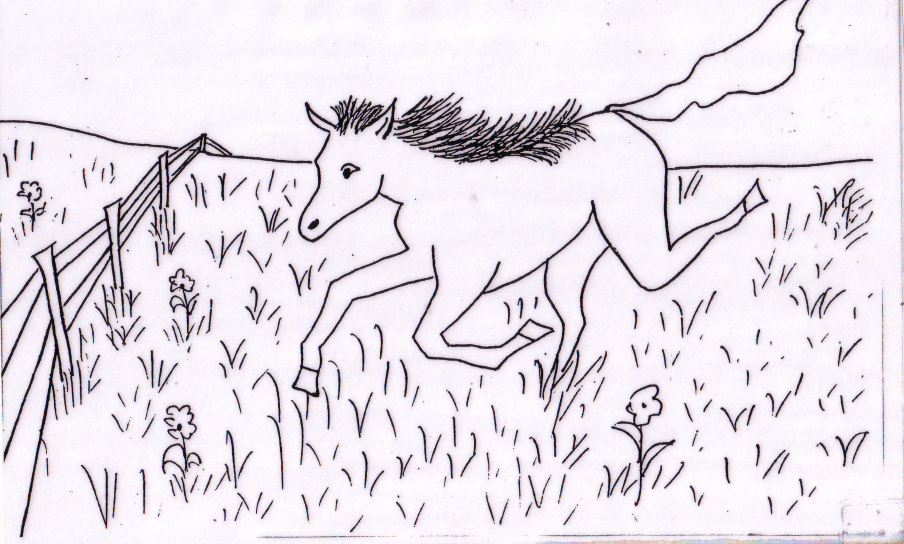
\includegraphics[width=2.4571in,height=1.4783in,width=\textwidth]{leclerq-img001.png}
 
\end{styleStandard}

\begin{styleStandard}
Picture 1
\end{styleStandard}

\begin{styleStandard}
  [Warning: Image ignored] % Unhandled or unsupported graphics:
%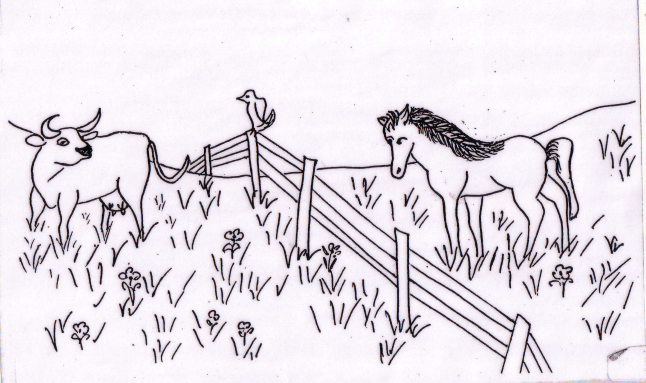
\includegraphics[width=2.4492in,height=1.452in,width=\textwidth]{leclerq-img002.png}
 
\end{styleStandard}

\begin{styleStandard}
Picture 2
\end{styleStandard}

\begin{styleStandard}
  [Warning: Image ignored] % Unhandled or unsupported graphics:
%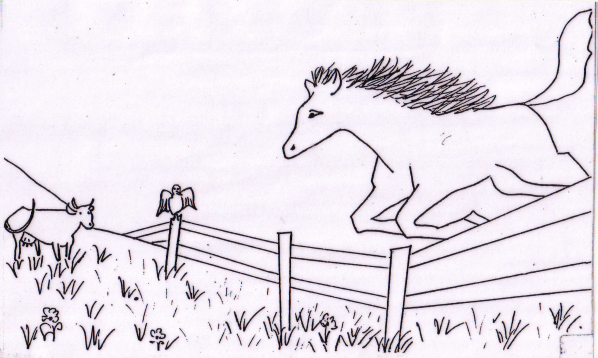
\includegraphics[width=2.4256in,height=1.452in,width=\textwidth]{leclerq-img003.png}
 
\end{styleStandard}

\begin{styleStandard}
Picture 3
\end{styleStandard}

\begin{styleStandard}
  [Warning: Image ignored] % Unhandled or unsupported graphics:
%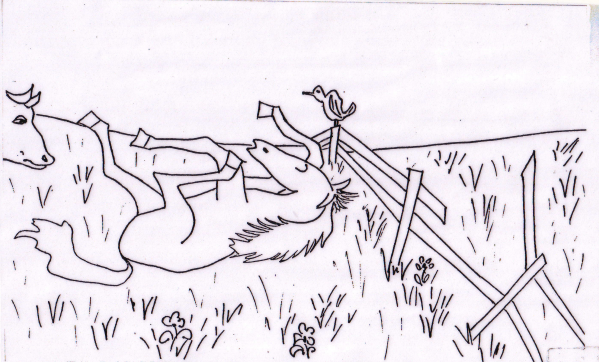
\includegraphics[width=2.4465in,height=1.4783in,width=\textwidth]{leclerq-img004.png}
 
\end{styleStandard}

\begin{styleStandard}
Picture 4
\end{styleStandard}

\begin{styleStandard}
  [Warning: Image ignored] % Unhandled or unsupported graphics:
%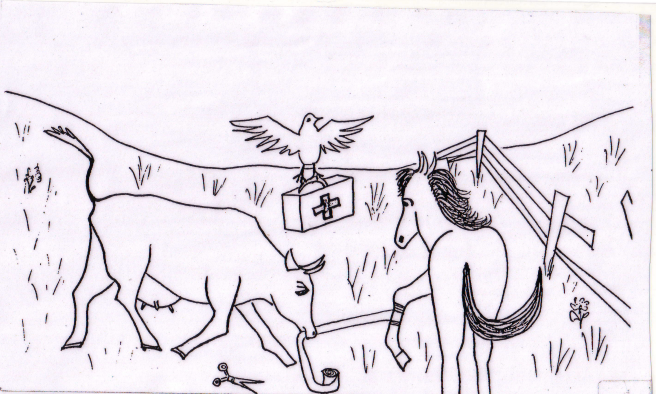
\includegraphics[width=2.4429in,height=1.4673in,width=\textwidth]{leclerq-img005.png}
 
\end{styleStandard}

\begin{styleStandard}
Picture 5
\end{styleStandard}

\begin{styleStandard}
\textbf{References}
\end{styleStandard}

\begin{styleStandard}
Andersen, Roger W. \& Shirai, Yasuhiro. 1994. Discourse motivations for some cognitive acquisition principles. \textit{Studies in Second Language Acquisition} 16.133–156.
\end{styleStandard}

\begin{styleStandard}
Bartning, Inge \& Schlyter, Suzanne. 2004. Itinéraires acquisitionnels et stades de développement en français L2. \textit{French Language Studies} 14. 281–299.
\end{styleStandard}

\begin{styleStandard}
Bassetti, Benedetta \& Escudero, Paola \& Hayes-Harb, Rachel. 2015. Second language phonology at the interface between acoustic and orthographic input. \textit{Applied Psycholinguistics} 36. 1–6.
\end{styleStandard}

\begin{styleStandard}
Brissaud, Catherine \& Sandon, Jean-Michel. 1999. L'acquisition des formes verbales en /E/ à l'école élémentaire et au collège: entre phonographie et morphographie. \textit{Langue Française} 124. 40–57.
\end{styleStandard}

\begin{styleStandard}
Brissaud, Catherine \& Chevrot, Jean-Pierre \& Lefrançois, Pascale. 2006. Les formes verbales homophones en /E/ entre 8 et 15 ans: contraintes et conflits dans la construction des savoirs sur une difficulté orthographique. \textit{Langue française} 151. 74–93.
\end{styleStandard}

\begin{styleStandard}
Cook, Vivian (ed.). 2002. \textit{Portraits of the L2 user}. Clevedon: Multilingual Matters.
\end{styleStandard}

\begin{styleStandard}
David, Jacques \& Guyon, Odile \& Brissaud, Catherine. 2006. Apprendre à orthographier les verbes: le cas de l'homophonie des finales en /E/. \textit{Langue française} 151. 109–126.
\end{styleStandard}

\begin{styleStandard}
Detey, Sylvain \& Nespoulous, Jean-Luc. 2008. Can orthography in[FB02?]uence second language syllabic segmentation? Japanese epenthetic vowels and French consonantal clusters. \textit{Lingua} 118. 66–81.
\end{styleStandard}

\begin{styleStandard}
Dewaele, Jean-Marc. 2003. Compte-rendu - hommage: l'oeuvre de L. Selinker. \textit{Link }49. 153-159.
\end{styleStandard}

\begin{styleStandard}
Fayol, Michel \& Pacton, Sébastien. 2006. L'accord du participe passé : entre compétition de procédures et récupération en mémoire. \textit{Langue française} 151. 59-73.
\end{styleStandard}

\begin{styleStandard}
Flavell, John H. 1977. \textit{Cognitive development}. Englewood Cliffs, NJ: Prentice Hall.
\end{styleStandard}

\begin{styleStandard}
Gass, Susan M. \& Mackey, Alison. 2000. \textit{Stimulated recall methodology in second language research}. Mahwah, NJ: Lawrence Erlbaum.
\end{styleStandard}

\begin{styleStandard}
Granget, Cyrille. 2015. Pourquoi le présent n'est-il pas si simple d'un point de vue psycholinguistique? \textit{Language, Interaction and Acquisition} 6(1). 107-148.
\end{styleStandard}

\begin{styleStandard}
Gretsch, Petra \& Perdue, Clive. 2007. Finiteness in first and second language acquisition. In F. Planck \& I. Nikolaeva (eds),\textit{ Finiteness.} \textit{Theoretical and empirical foundations}, 432-484. Oxford: Oxford University Press.
\end{styleStandard}

\begin{styleStandard}
Han, ZhaoHong \& Tarone, Elaine. 2014. Introduction. In Z. Han, E. Tarone (ed.), \textit{Interlanguage. Forty years later}, 1-6. Amsterdam: John Benjamins Publishing Company.
\end{styleStandard}

\begin{styleStandard}
Hawkins, Roger. 2004. The contribution of the theory of Universal Grammar to our understanding of the acquisition of French as a second language. \textit{French Language Studies} 14. 233–255.
\end{styleStandard}

\begin{styleStandard}
Hendriks, Henriëtte. 1998. Comment il monte le chat ? en grimpant !~\textit{Acquisition et interaction en langue étrangère} 11. (\url{http://journals.openedition.org/aile/1454}\textstyleListLabellxx{). (}Accessed 2019-04-09.)
\end{styleStandard}

\begin{styleStandard}
Herschensohn, Julia. 2001. Missing inflection in second language French: accidental infinitives and other verbal deficits. \textit{Second Language Research} 17(3). 273-305.
\end{styleStandard}

\begin{styleStandard}
Hickmann, Maya. 1982. \textit{The development of narrative skills: Pragmatic and metapragmatic aspects of discourse cohesion.} Chicago: University of Chicago. (Doctoral dissertation)~
\end{styleStandard}

\begin{styleStandard}
Hickmann, Maya \& Hendriks, Henriëtte \& Roland, Françoise. 1998. Référence spatiale dans les récits d'enfants français : perspective inter-langue. \textit{Langue française} 118. 104-123.
\end{styleStandard}

\begin{styleStandard}
Hickmann, Maya \& Hendriks, Henriëtte \& Demagny, Annie-Claude \& Engemann, Helen \& Iakovleva, Tatiana \& Ji, Yinglin \& Ochsenbauer, Anna-Katharina \& Soroli, Efstathia. 2011. \textit{La représentation de l'espace - études expérimentales et translinguistiques - Vol 1. Manuel de codage}. Université Paris 8.
\end{styleStandard}

\begin{styleStandard}
Hilton, Heather. 2014. Oral Fluency and Spoken Proficiency: Considerations for Research and Testing. In Leclercq, P., A. Edmonds \& H. Hilton (eds.), \textit{Measuring L2 proficiency: perspectives from SLA,} 27-53. Bristol: Multilingual Matters.
\end{styleStandard}

\begin{styleStandard}
Jaffré, Jean-Pierre. 2006. Pourquoi distinguer les homophones ? \textit{Langue française} 151. 25-40.
\end{styleStandard}

\begin{styleStandard}
Jefferson, Gail. 1996. A case of transcriptional stereotyping. \textit{Journal of Pragmatics} 26. 159-170.
\end{styleStandard}

\begin{styleStandard}
Keysar, Boaz \& Lin, Shuhong \& Barr, Dale J. 2003. Limits on theory of mind use in adults. \textit{Cognition} 89. 25-41.
\end{styleStandard}

\begin{styleStandard}
Klein, Wolfgang. 1994. \textit{Time in Language}. Routledge.
\end{styleStandard}

\begin{styleStandard}
Klein, Wolfgang. 2006. On finiteness. In V. Van Geenhoven (ed.), \textit{Semantics in Acquisition,} 245-272. Dordrecht: Springer.
\end{styleStandard}

\begin{styleStandard}
Klein, Wolfgang \& Perdue, Clive. 1989. The learner’s problem of arranging words. In. Bates, E., B. MacWhinney (eds.), \textit{The cross-linguistic study of sentence processing,} 292-327. Cambridge: Cambridge University Press.
\end{styleStandard}

\begin{styleStandard}
Kormos, Judit. 2006. \textit{Speech Production and Second Language Acquisition}. Mahwah, NJ: Lawrence Erlbaum.
\end{styleStandard}

\begin{styleStandard}
Lardiere, Donna. 2012. Linguistic approaches to second language morphosyntax. In Gass, S. M., Mackey, A. (eds.), \textit{The Routledge Handbook of Second Language Acquisition}, 106-126. Oxon: Routledge.
\end{styleStandard}

\begin{styleStandard}
Leclercq, Pascale. 2011. How do learners of French and English include space and time reference in narratives? (Paper presented at the EUROSLA 21 conference, Stockholm, 8-10 September 2011).
\end{styleStandard}

\begin{styleStandard}
Lenart, Ewa \& Perdue, Clive. 2004. L’approche fonctionnaliste : structure interne et mise en œuvre du syntagme nominal.~\textit{Acquisition et Interaction en Langue Etrangère}~21. 85-121.
\end{styleStandard}

\begin{styleStandard}
Leow, Ronald P. \& Morgan-Short, Kara. 2004. To think aloud or not to think aloud: The Issue of Reactivity in SLA Research Methodology.~\textit{Studies in Second Language Acquisition}~26(1). 35-57.
\end{styleStandard}

\begin{styleStandard}
Mackey, Alison, \& Gass, Susan. 2012. \textit{Research Methods in Second Language Acquisition: a practical guide.} Chichester: Blackwell Publishing.
\end{styleStandard}

\begin{styleStandard}
MacWhinney, Bryan. 2000. \textit{The CHILDES Project: Tools for Analyzing Talk}. 3rd Edition. Mahwah: Lawrence Erlbaum Associates.
\end{styleStandard}

\begin{styleStandard}
Mondada, Lorenza. 2000. Les effets théoriques des pratiques de transcription. \textit{Linx} 42. 131-146.
\end{styleStandard}

\begin{styleStandard}
Mondada, Lorenza. 2002. Transcrire l’interaction. \textit{Cahiers de Praxématique} 39. 45-75.
\end{styleStandard}

\begin{styleStandard}
Mondada, Lorenza. 2007. Commentary: transcript variations and the indexicality of transcribing practices. \textit{Discourse Studies} 9(6). 809-821.
\end{styleStandard}

\begin{styleStandard}
Myles, Florence \& Hooper, Janet \& Mitchell, Rosamond .1998. Rote or rule? Exploring the role of formulaic language in classroom foreign language learning. \textit{Language Learning} 48(3). 323–364.
\end{styleStandard}

\begin{styleStandard}
Nickerson, Raymond S. 1999. How we know - and sometimes misjudge - what others know: imputing one's own knowledge to others. \textit{Psychological Bulletin} 25(6). 737-759.
\end{styleStandard}

\begin{styleStandard}
Nimz, Katharina \& Khattab, Ghada. 2019. On the role of orthography in L2 vowel production: The case of Polish learners of German. \textit{Second Language Research}. 1 –30.
\end{styleStandard}

\begin{styleStandard}
Norris, John M. \& Ortega, Lourdes. 2012. Assessing learner knowledge. In Gass, S.M. \& Mackey, A. (eds.), \textit{The Routledge Handbook of Second Language Acquisition}, 573-589. Oxon: Routledge. 
\end{styleStandard}

\begin{styleStandard}
Noyau Colette \& Houdaïfa, Et-Tayeb \& Vasseur, Marie-Thérèse \& Véronique, Georges Daniel. 1995. The acquisition of temporality in French. In Dietrich, R., W. Klein \& C. Noyau (eds.), \textit{The acquisition of temporality in a second language}, 145-210. Amsterdam: John Benjamins Publishing Company. 
\end{styleStandard}

\begin{styleStandard}
Ochs, Elinor. 1979. Transcription as theory. \textit{Developmental pragmatics} 10(1). 43-72. 
\end{styleStandard}

\begin{styleStandard}
Ortega, Lourdes. 2014. Trying out theories on interlanguage: Description and explanation over 40 years of L2 negation research. In Han, Z., E. Tarone (eds.), \textit{Interlanguage: Forty years later,} 173-201. Amsterdam: John Benjamins Publishing Company.
\end{styleStandard}

\begin{styleStandard}
Pallotti, Gabriele. 2017. Applying the interlanguage approach to language teaching. \textit{International Review of Applied Linguistics} 55(4). 393-412.
\end{styleStandard}

\begin{styleStandard}
Perdue, Clive \& Benazzo, Sandra \& Giuliano, Patrizia. 2002. When finiteness gets marked: the relation between morphosyntactic development and use of scopal items in adult language acquisition. \textit{Linguistics} 40(4). 849-890.
\end{styleStandard}

\begin{styleStandard}
Prévost, Philippe. 2007a. L'influence du paradigme verbal de la langue maternelle sur la variabilité morphologique en acquisition du français L2 par des apprenants adultes. \textit{French Language Studies} 17. 49-80.
\end{styleStandard}

\begin{styleStandard}
Prévost, Philippe. 2007b. Knowledge of morphology and syntax in early adult L2 French: Evidence for the missing surface in[FB02?]ection hypothesis. In Goodluck, H., J. M. Liceras et H. Zobl (eds.), \textit{The Role of Formal Features in Second Language Acquisition, }353-377. Mahwah, NJ: Lawrence Erlbaum. 
\end{styleStandard}

\begin{styleStandard}
Prévost, Philippe \& White, Lydia. 2000. Missing Surface Inflection or Impairment in second language acquisition? Evidence from tense and agreement. \textit{Second Language Research} 16(2). 103–133.
\end{styleStandard}

\begin{styleStandard}
Revesz, Andrea. 2012. Coding Second Language Data Validly and Reliably. In Mackey, A., S. Gass, \textit{Research Methods in Second Language Acquisition: a practical guide}, 203-221. Chichester: Blackwell Publishing.
\end{styleStandard}

\begin{styleStandard}
Robison, Richard E. 1995. The aspect hypothesis revisited: a cross-sectional study of tense and aspect marking in interlanguage. \textit{Applied Linguistics} 16. 344-370.
\end{styleStandard}

\begin{styleStandard}
Rohde, Andrea. 1996. The aspect hypothesis and the emergence of tense distinction in naturalistic L2 acquisition. \textit{Linguistics} 34. 1115-1137.
\end{styleStandard}

\begin{styleStandard}
Saturno, Jacopo. 2015. La trascrizione di varietà di apprendimento iniziali. In Chini, M. (ed.), \textit{Il parlato} \textit{in [italiano] L2: aspetti pragmatici e prosodici. [Italian] L2 Spoken Discourse: Pragmatic and Prosodic Aspects}, 117-138. Milano: FrancoAngeli.
\end{styleStandard}

\begin{styleStandard}
Selinker, Larry. 1972. Interlanguage. \textit{International Review of Applied Linguistics} 10. 219-231.
\end{styleStandard}

\begin{styleStandard}
Véronique, Daniel. 2004. The development of referential activities and clause-combining as aspects of the acquisition of discourse in French as L2. \textit{French Language Studies} 14. 257–280.
\end{styleStandard}
\end{document}
